%=========================================================================
% (c) Michal Bidlo, Bohuslav Křena, 2008

\chapter{Úvod}
V minulosti v oblasti herného priemyslu existovalo niekoľko poskytovateľov, ktorý sprostredkovali rôzne služby pre vývojárov hier, ako napríklad tabuľky online hráčov, správa odmien, pokročilé štatistiky prístupov, alebo vlastné štatistiky. Tieto služby boli orientované iba na webové flash hry a aj väčšina z tých pomaly zaniká, alebo už zanikla pomaly upadajúcou technológiu flash. Za zmienku stojí napríklad leader sveta flashových hier menom Mochimedia. S rozmachom moderných webových technológií a príchodom HTML5/Javascript hier dlho neexistovala žiadna webová stránka ponúkajúca podobné vyššie zmienené služby. Príchodom webového portálu clay.io v roku 2012 sa vývojárov javascriptových hier usmialo štastie. Clay.io ponúkalo rôzne služby pre herných vývojárov, bez nutnosti mať státisíce prístupov do hry, alebo mať hru špičkovej úrovni. Služby boli dostupné pre všetkých bez rozdielu. Avšak začiatkom roka 2015 sa clay.io začalo orientovať iným smerom a z tejto webovej služby sa stal viac portál pre hráčov ako pre vývojárov. Už viac nebolo možné integrovať API, do hociktorej hry a všetky hry, ktoré chceli byť umiestnené na portáli clay.io a využívať jeho služby boli vyberané podľa kvality. Taktiež hry využívajúce API bolo možné hrať iba na webe clay.io a developer nesmel distribuovať hru na iných webových portáloch. Týmto sa clay.io uzavrelo a zaradilo sa vedľa iných svetových distribútorov HTML5 hier, ako napríklad Boostermedia, Softgames, alebo Spilgames.

Táto bakalárska práca vznikla z dôvodu neexistenice otvoreného modernej webovej platformy na tvorbu hier pre všetkých bez rozdielu a služby ponúkajúc zadarmo. Táto webová platforma by mala byť orientovaná nielen na vývojárov javascriptových hier, ktorý prostredníctvom API by mali možnosť využívať služby platformy, ale aj na hráčov týchto vytvorených hier. Hráči by mali byť schopný hrať hry na akejkoľvek platforme, či už desktopových osobných počítačoch, alebo moderných chytrých telefónoch. Z toho dôvody by mala minimálne časť webového portálu určená hráčom byť do určitej miery responzivna.

Nasledujúca kapitola sa venuje predstaveniu technológiam, ku ktorým sa dostalo a následne boli využité v rámci vypracovania tejto práce. Ďalšia kapitola sa venuje návrhu celého webového portálu a API. Po návrhu prišla na rad implementácia, o ktorej je písané v rovnako pomenovanej kapitole. A nakoniec celá webová platforma bola zverejnená a testovaná v reálnych podmienkach. O tejto fázi hovorí kapitola testovanie.

\chapter{Použité technológie}
Pri implementácií platformy bolo nutné si dobre premyslieť čo bude potreba a špecifikovať požiadavky na technológie, ktoré sa budú využívať. Keď sa zhrnuli všetky požiadavky, tak z toho vyšlo, že je potreba programovací jazyk pre serverovú časť, klientskú časť, jazyk pre API pre vývojárov, databázu a databázový jazyk a jazyk, v ktorej bude napísaná hra demonštrujúca funkcie webovej platformy.

\section{Serverová časť}
Pod pojmom serverová časť sa myslí všetko to, čo sa vykonáva na servery. Teda v prípade tejto práce to je hlavne generovanie webovej stránky platformy a práca s datami úložených v databázi. Okrem týchto vecí sa používa serverová časť pri práci s API, kedy sa využíva AJAX.

Pri výbere jazyka pre serverovú časť sa ponúkalo hneď niekoľko možností. Bolo na výber medzi PHP, Python, Java, Ruby, alebo ASP . NET. Zavážili hlavne vlastnosti, ktoré sú spomenuté v nasledujúcej kapitole.
 

\subsection{PHP}
Hypertext Preprocessor je široko používaný a univerzálny open source skriptovací jazyk, ktorý sa obzvlášť používa na vývoj webových apolikácií a je možné ho vložiť do HTML súboru. Syntax jazyka je veľmi podobná syntaxe jazyku C, taktiež veľa vlastností prebral zo skriptovacieho jazyka Perl. Od novších vydaní je v PHP taktiež možnosť používania objektov. Tento skripotvací jazyk beží takmer na všetkých operačných systémoch od UNIXu cez Windows až po MAC OS X.

PHP bol zvolený pre serverovú časť hlavne vďaka tomu, že to je najrozšírenejší serverový jazyk a takmer všetci poskitovatelia hostingu ponúkajú hosting práve s PHP. Okrem toho sa v PHP ľahko pracuje s relačnými databázami, a hlavne s MySQL, ktorému sa venuje kapitola.

\subsection{Model Controler View architektúra}
Základnou myšlienkou architektury MVC je oddelenie 	logiky od výstupu. MVC, jako už názov napovedá pozostáva z 3 typov komponent, z modelu, pohľadu (view) a kontroleru. Model obsahuje všetku logiku aplikácie, môžu sa v ňom nachádzať například výpočty alebo databázové operácie. Komponenta pohľad sa zase stará o zobrazovanie vústupu užívateľovi. Obsahuje minimálne množství logiky, ktorá je pre výpis nutná. Tretí a posledný typ je kontroler, ktorý komunikuje s užívateľom, modelom aj pohľadom a komponenty navzájom prepája. Príklad takéjto architektury a komunikácií medzi jednotlivými komponentami je zobrazený na nasledujúcom obrázku.
\begin{figure}[h]
  \centering
  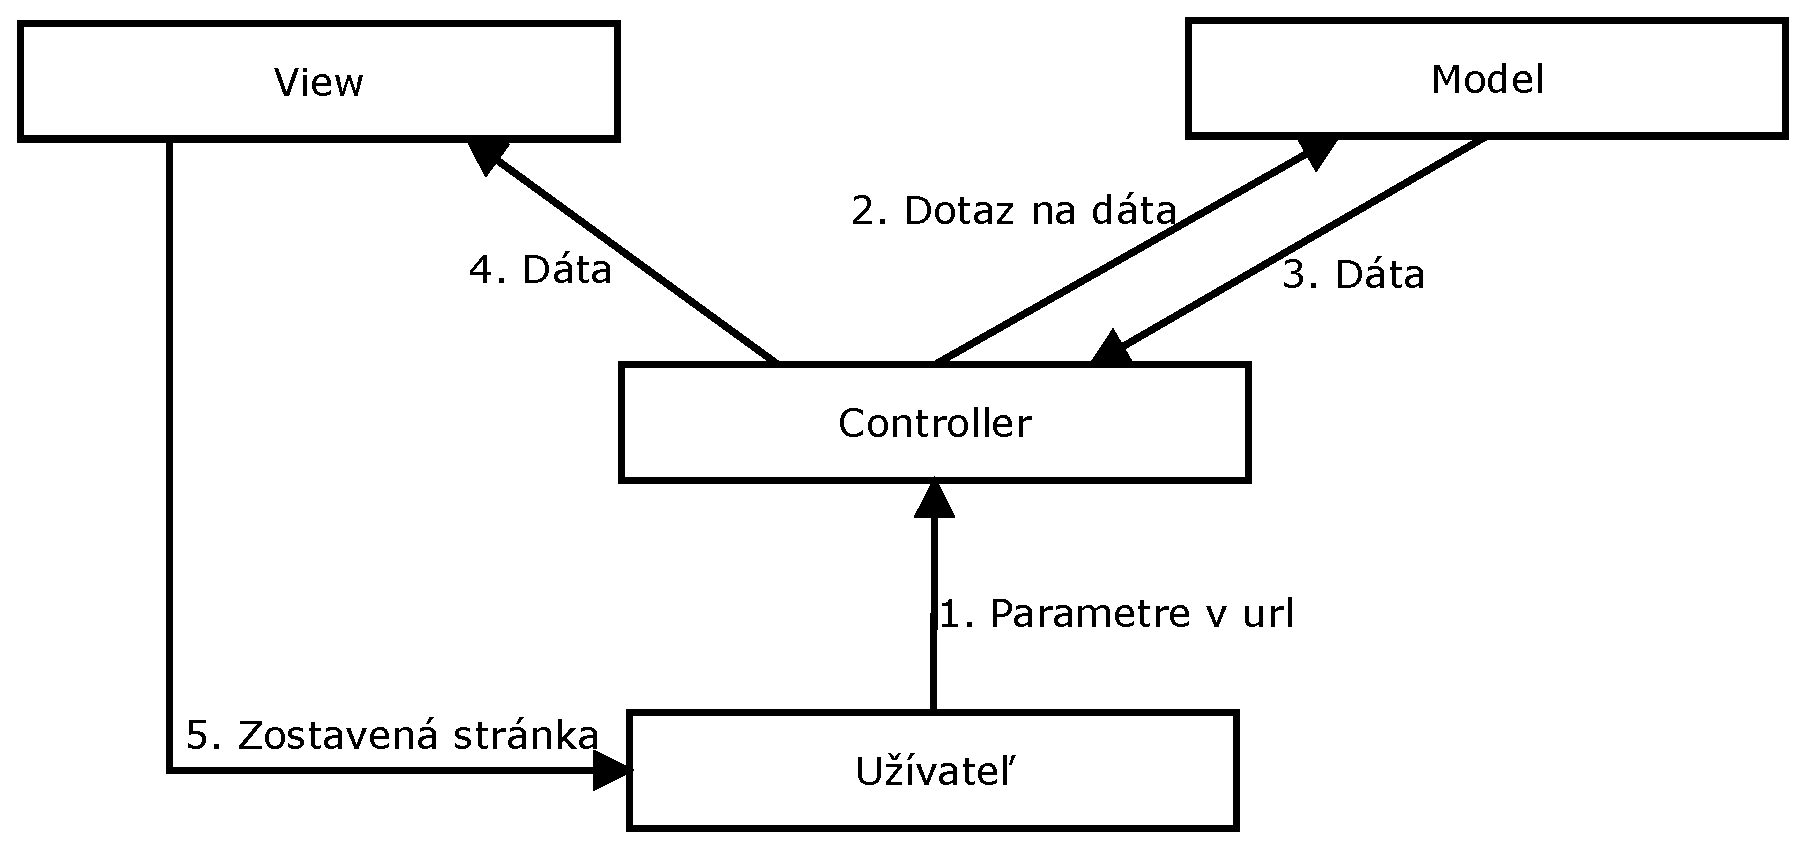
\includegraphics[scale=0.35]{fig/mvc.eps}
  \caption{MVC architektúra}
  \label{fig:mvc}
\end{figure}

\subsection{Nette}
Už PHP je samo o sebe mocný programovací jazyk, ale ak by bolo zvolené čisté PHP, tak by programátol musel riešiť veľké množstvo vecí, ktoré niekto v minulosti už dávno vyriešil. Okrem toho by si programátor musel dávať veľký pozor a ošetrovať početné množstvo bezpečnostných rizík. Kvôli týmto spomenutým veciam bol pre účel práce vybraný rámec Nette.

Nette je rámec pre tvorbu webových aplikácií v PHP5, ktorý sa zameriava na elimináciu bezpečnostných rizík, podporuje AJAX a MVC. Z veľkej časti je založený na použití komponentov. Pôvodným autorom je David Grundl, ale v súčasnosti sa o rozvoj rámcu stará Nette Foundation. Je ponúkaný pod licenciou GNU GPL a licenciou Nette (obdoba BSD licencie). Rámec sa teší veľkej obľube a taktiež početnej komnuite v Čechách a na Slovensku.

Minimálne požiadavky, pre funkčnosť sa vyžaduje PHP verzie 5.3.1 a vyššej a v tomto prípade MySQL verzie 5.6. Tieto požiadavky je možné overiť oficiálnym requirements-checker.php skriptom.


\section{Databázová časť}
Pre uloženie a uchovávanie dát bola zvolená relačná databáza. Databáza bola zvolená hlavne kvôli vlastnosti ACID a pre prístup pre viacerých užívateľov k databázi súčastne. Okrem iného databáze šetria pamäťové miesto tým, že pri dobrom návrhu sa v databázi nenachádzajú redundantné dáta. Na výber boli rôzne alternatívy ako napríklad PL/SQL, T-SQL alebo vybraný MySQL.  

\subsection{MySQL}
MySQL je otvorený viacužívateľský SQL relačný databázový server, ktorý je implementovaný vo viacerých programovacích a jlavne serverových jhazykoch. Príkladosm je skriptovací jazyk PHP. Je to databázový relačný systém, teda každá databáza v MySQL je tvorená z jendnej alebo viacerých tabuliek, ktoré majú riadky a stĺpce. Riadky udávajú jendotlivé záznamy, stĺpce zase dátový typ jednotlivých záznamov. Práca s takouto databázou je vykonávaná pomocou takzvaných dotazov.

\section{Klientská časť}
Klientská časť pokrýva všetko to čo je zobrazené užívateľovi, teda kompletná stránka, ktorej zostavovanie sa dialo z väčšej miery na servery. Aby boli ibnformácie určené pre užívateľa zobrazené v nejakej prijatelnej a užívateľsky prívetivej podobe, tak je dobrým zvykom okrem značkovacieho jazyka HTML použiť aj CSS kaskádové štýly. Keďže moderná prezentácia informácií na webových portáloch vyžaduje aj určitú ľahkosť a dynamiku, tak k tomuto účeľu bol použitý celosvetovo rozšírený programovací jazyk Javascript.

\subsection{HTML}
Hyper Text Markup Language je značkovací jazyk určený pre popis webových dokumentov, hlavne teda webových stránok. Najskôr bol iba veľmi jendoduchá podmnožina jazyka SGML, ale neskôr sa z neho vyvinul samostatný štandart. HTML dokument sa popisuje pomocou HTML tagov, každý typ HTML tagu popisuje odlišný obsah dokumentu.  

V minulosti sa HTML používal aj na definovanie štruktúry dokumentu a aj jeho výzoru. V súčastnej dobe je HTML určené iba na zmienenú definíciu dokumentu.

\subsection{CSS}
Kvôli okolnostiam, spomenutých na konci kapitoli, bol vyvynutí Cascading Style Sheets. CSS popisuje ako budú HTML tagy zobrazené na obrazovke, papiery, alebo inom médiu. CSS šetrí veľa času tým, že môže popisovať rozmiestnenie viacerých webových stránok naraz.

\subsection{Javascript}
Javascript je skriptovací protoypovo založený jazyk, ktorý sa v súčastnosti používa hlavne pri tvorbe webových prezentácií a stránok. Javascript beží na klientskej strane webu, teda je spúštaný väčšinou vo webových prehliadačoch používateľov. V súčastnosti Javascript popdoruje väčšina webových prehliadačov a zároveň je najpoužívanejší skriptovací jazyk používaný na klientskej strane.

Bola by chyba myslieť si, že Javascript svoje uplnatnenie pri tvorbe webov má iba na strane klienta. Javascript je naozaj všestranný jazyk a svoje uplatnenie nájde aj na servery v podobe Node.js. Pre účely tejto práce je avšak použitý klasický klientský javascript spúštaný vo webovom prehliadači.


\subsection{JQuery}
JQuery je ľahká a rýchla Javascriptová knižnica, ktorá kladie dôraz na interakciu medzi Javascriptom a HTML. Syntax knižnice je navrhnutá tak, aby bolo používanie Javascriptu na stránke jendoduchšie. Medzi hlavné zjednodušenia oproti čistému Javascriptu patrí: navigácia dokumentu, výber DOM elementov, vytváranie animácií, spracovanie udalostí a veľa iných nie menej podstatných vecí. Knižnica zároveň rieši tzv. cross-browser problémy, kedy jedna věc sa môže v rôznych prehliadačoch správať odlišne.
JQuery je zároveň najobľúbenejšia a najrozšírenejšia Javascriptová knižnica, o čom svedčí nielen početná komunita, ale aj to, že je využívaná najväčšími firmami jako Google, či Microsoft.


\subsection{Bootstrap}
Bootstrap je frontendový rámec pre rýchle a ľahké vyvíjanie webov. Obsahuje dizajnérske typografické šablóny založené na HTML a CSS, napríklad formuláre, tlačítka, modálne okná a mnohé iné. Okrem toho, umožnuje ľahko tvoriť responzivny dizajn. Hodí sa predovšetkým na protoypovanie stránky, hlavne kvôli značnej neoriginálnosti, pretože väčšina stránok založená na tomto rámci vypadá veľmi podobne. Avšak jendoduchými   modifikáciami si skúsený dizajnér upraví Bootstrap k svojmu obrazu.  

\subsection{Chart.js}
Javascriptová knižnica, pomocou ktorej je tvorba grafov z daných dát veľmi jhendoduchá. Na zobrazovanie grafov používa HTML tag <canvas >. Na výber je z 6 najbežnejších typov grafov. Takto vytvorené grafy sú plne responzivne, takže môžu byť správne zobrazené ako na stolných počítačoch s veľkou obrazovkou, tak aj na malých mobilných zariadeniach.

\section{API}
API je v tomto prípade myslená, ako knižnica, pomocou ktorej vývojári hier pristupujú k funkciám webovej platformy. Knižnica je implementovaná v Javascripte a k funkciám platformy, ktoré sú na servery sa pristupuje pomocou dotazovaním technológiou AJAX.

\subsection{AJAX}
Asynchronous Javascript and XML je súhrné označenie technológie, ktorá umožňuje meniť obsah stránok bez toho, aby bolo nutné ich celé znova načítať zo servera. Hlavná výhoda spočíva v tom, že sa prenáša značne menšie množstvo dát. AJAX nieje samostatný programovací jazyk ani technológia sama o sebe, ako by sa mohlo zdať, je to skôr kombinácia niekoľkých prvkov. Je založený na internetových štandardoch, a používa kombináciu HMLHttpRequest pre získanie dát zo servera a Javascript/DOM pre zobrazenie a použitie dát. Väčšinou sa používa spolu s Javascriptom, ale nie je to podmienka, lebo je podporovaný aj v iných programovacích jazykoch.  
\begin{figure}[h]
  \centering
  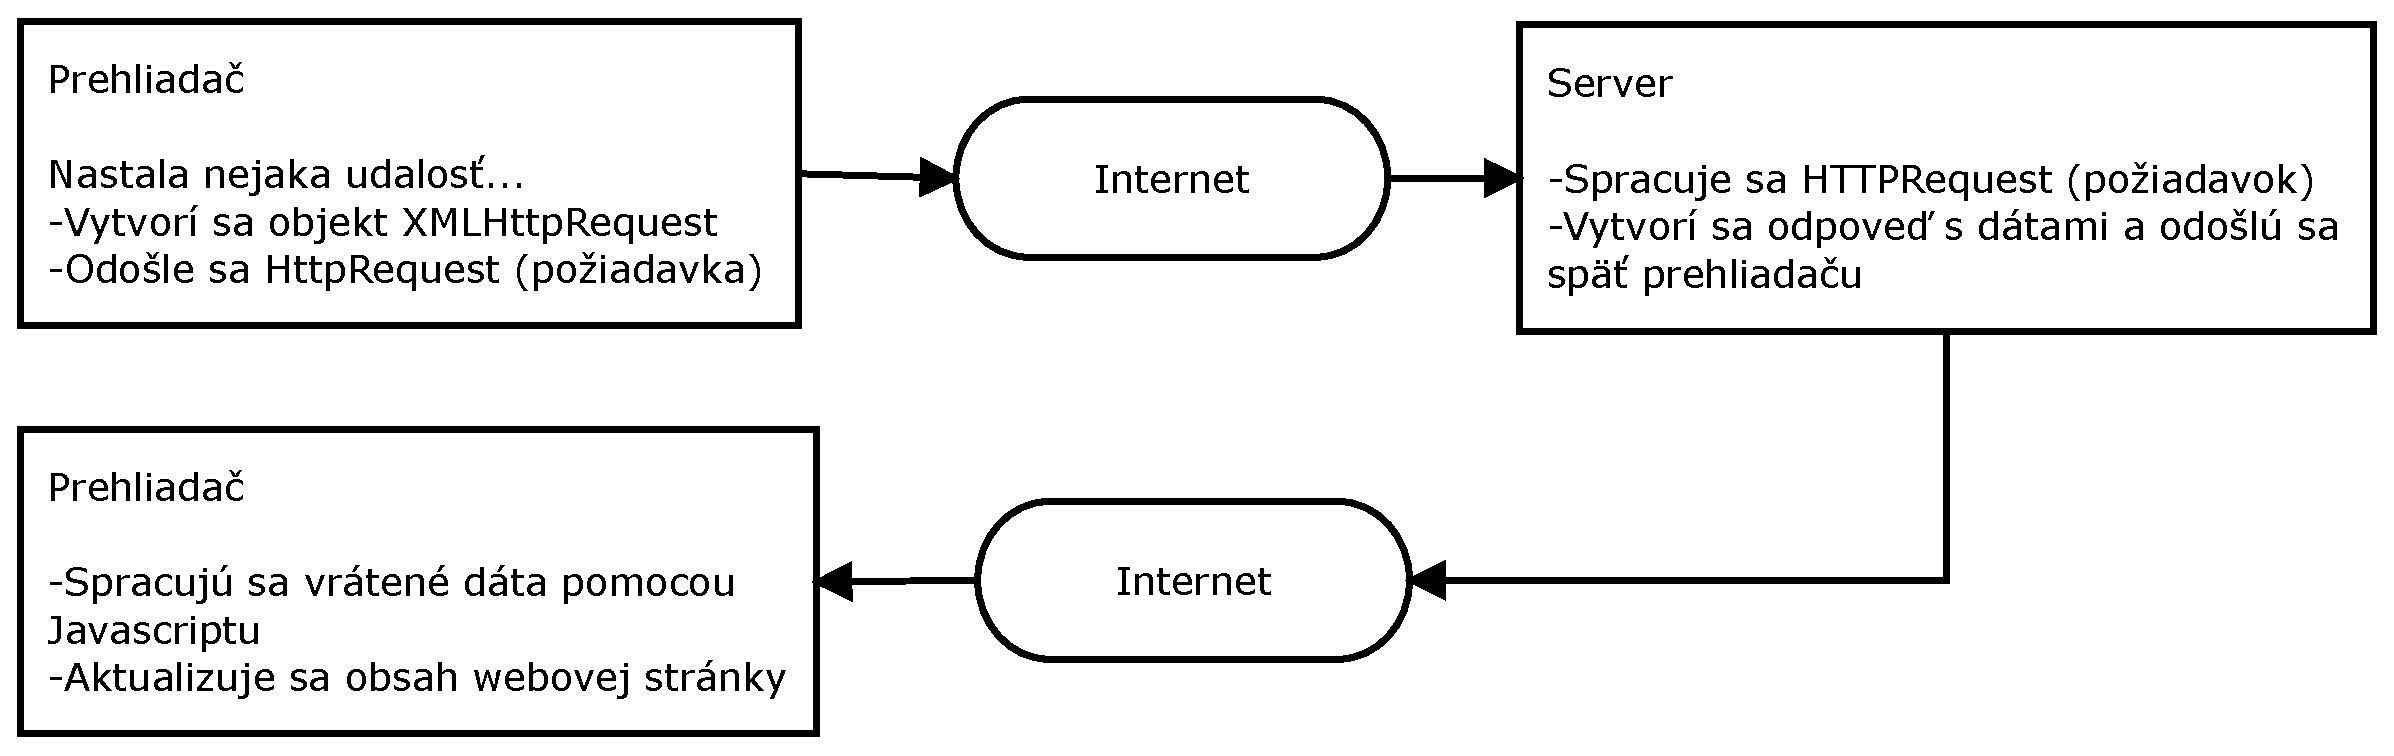
\includegraphics[scale=0.35]{fig/ajax.eps}
  \caption{Neblokujúca komunikácia so serverom pomocou AJAXu}
  \label{fig:ajax}
\end{figure}

\subsection{CORS}
Klasický javascript je limitovaný tzv. Same origin policy, z toho dôvodu nie je možné prijímať odpoveďe z domény, keď stránka, alebo hra, ktorá požiadavok má inú doménu. 

Tento známy, hore popísaný problém rieši Cross-origin resource sharing. CORS je vlastne mechanizmus, ktorý povoluje zakázané zdroje na webovej stránke aby boli požiadané z inej domény ako z domény z ktorej zdroje pochádzajú. Pre použitie tohto mechanizmu musí nastať zmena pri tvorbe požiadavku na klientovi, a je treba povoliť CORS na servery. Prehliadač musí posielať nastavenie Origin: doména v http hlavičke. Na servery zase musí byť nastavené povolenie Acces-Control-Allow-Origin: * (* znamená že budú povolené všetky domény).

\section{Hra}
Pre demonštračnú hru sa ponúkalo buďto použiť klasický Javascript, čo ale nie je príliš rozšírená forma tvorby HTML5 hier, alebo použiť jeden z početného množstva rámcov, ktoré sú určené špeciálne na tvorbu hier. Na výber bol Ease.js, Tree.js, Panda.js, melon.js, Kiwi.js alebo Phaser.js a mnoho ďalších. Výber padol práve na Phaser.js, pretože to je jeden z najpoužívanejších a najbežnejších Javascriptových rámcov, určených pre programovanie hier, o čom svečí hlavne početná komunita okolo tohto rámca a fakt, že aj mnohé firmy z oblasti herného byznisu, ako Boostermedia pracujú práve s týmto rámcom. 

\subsection{Phaser}
Phaser je javascriptový rámec určený špeciálne pre tvorbu hier (aj desktopových, aj mobilných), ktorý je založený na renderovacom rámci pixi.js. Phaser je ľahko naučiteľný, rýchly, je ponúkaný zadarmo a má otvorený kód. Podporuje ako canvas, tak aj webgl. Obshauje veľké množstvo predpripravených funkcií a spracovaných tak aby ich použitie bolo jendoduché. Príkladom môže byť stavaný preloader, fyzika, sprity, animácie, častice, rôzne módy prisposobenia veľkosti obrazovky a iné. 

\chapter{Analýza existujúcich riešení}
todo

\section{Herné služby}
todo

\subsection{Google Play Game Services}
todo

\subsection{Apple Game Center}
todo

\subsection{Mochimedia}
todo

\subsection{Clay.io}
todo

\subsection{Steam}
todo

\section{Znovupoužiteľné komponenty}
todo

\subsection{Odmeny}
todo

\subsection{Tabuľky najlepších hráčov}
todo

\subsection{Štatistiky}
todo

\subsection{Úložisko v cloude}
todo

\chapter{Návrh riešenia}
todo

\chapter{Implementácia}
todo

\chapter{Testovanie}
todo

\chapter{Záver}
todo












%=========================================================================
